% ----------------------------------------------------------
\chapter{Physics-Informed Learning}\label{ch:pinn}
% ----------------------------------------------------------

Solving an \gls{IVP} for \gls{ODE}s using deep learning is not as straight-forward as it may seem.
Indeed, it falls under the function approximation paradigm, in which we want to train a deep learning model to approximate a target function (which is the solution to the \gls{IVP}).
In this scenario, it is usual that either the target function is unknown or it is too complex to be useful, and, thus, only input-output samples are available to train the deep learning model.
This is the case for most of the well-known successful applications of deep learning, such as those involving computer vision and the classification of images. % TODO find sources

However, that is not the case for \glspl{IVP}.
When a solution for an \gls{IVP} is desired, the target function is not known, but neither are the input-output pairs.
Actually, generating such training data is essentially solving the \gls{IVP}.
Yet, the \emph{dynamics} of the solution is usually well-known, in the form of an \gls{ODE}.
This chapter focuses on communicating an approach to harvest this knowledge efficiently and to use it to train deep feedforward networks that approximate the solution of \glspl{IVP}.
More specifically, the work of \textcite{Raissi2019} is presented in a more limited formulation, targeting \gls{ODE}s\footnotemark.
\footnotetext{The original work focuses on partial differential equations, having \gls{ODE}s as a particular case.}

\section{Problem Statement}\label{sec:pinn-problem}

Let us first recall the \gls{IVP}.
Given an \gls{ODE} (written like in Equation \eqref{eq:ode}) and boundary conditions, we want to find a solution that satisfies both.
More precisely, given $\mathcal{N}:\R\times \R^m\to \R^{m}$ and initial conditions $t_0\in I\subset \R,\,\bm{y}_0\subset \R^{m}$, we want to find $\bm{\phi}:I\to \R^{m}$ such that
\begin{align*}
    \frac{d \bm{\phi}(t)}{d t} &= \mathcal{N}\left( t, \bm{\phi}(t) \right),\,t\in I \\
    \bm{\phi}(t_0) &= \bm{y}_0
.\end{align*}

Solving this using deep feedforward networks means to train a model $D^{FN}_{\gls{param}}:I\to \R^{m}$, parametrized by $\gls{param}\in \Omega$, that satisfies the same conditions, i.e.,
\begin{align}
    \frac{d D^{FN}_{\gls{param}}(t)}{d t} &= \mathcal{N}\left( t, D^{FN}_{\gls{param}}(t) \right),\,t\in I \label{eq:dl-ode} \\
    D^{FN}_{\gls{param}}(t_0) &= \bm{y}_0 \label{eq:dl-ivp}
.\end{align}

The naïve approach would be to construct a set $X=\left\{ (t,\bm{y})\in I\times \R^{m}: \bm{y}=\bm{\phi}(t) \right\} $ to be used as the experience for the learning algorithm.
Then, with a properly constructed cost function and given that the model is complex enough, the model $D^{FN}_{\gls{param}}$ would approximate the target $\bm{\phi}$ and, by consequence, satisfy Equation \eqref{eq:dl-ode} and Equation \eqref{eq:dl-ivp}.
However, note how this approach assumes that $\bm{\phi}$ is known, as it is required to construct a set $X$ with more than just $\left( t_0,\bm{y}_0 \right) $.
Therefore, in many \gls{IVP} setups, training a deep learning model this way would either be impossible or useless.

\section{Physics Regularization}\label{sec:PI}

The naïve approach described above is quite inefficient in that it does not use the information provided by the known $\mathcal{N}$ function.
This is precisely the turning point for making deep learning a viable option in solving \gls{IVP}s.
The approach of \textcite{Raissi2019} proposes to train the model using a regularization based on $\mathcal{N}$.
This means to train $D^{FN}_{\gls{param}}$ to approximate $\bm{\phi}$ at the initial condition (since this is known by the definition), satisfying Equation \eqref{eq:dl-ivp}, but also to train its Jacobian to approximate $\mathcal{N}$, satisfying Equation \eqref{eq:dl-ode}.

For this, let us define the singleton $X_b=\left\{ \left( t_0,\bm{y}_0 \right)  \right\} $ and the set $X_{\mathcal{N}}=\left\{ t\in I \right\} $. Then, we can construct \[
    J_b\left( \gls{param} \right) = \sum_{\left( t,\bm{y} \right) \in X_b } \|D^{FN}_{\gls{param}}(t) - \bm{y}\|_2 = \|D^{FN}_{\gls{param}}\left( t_0 \right) -\bm{y}_0\|_2
,\] which looks like a usual cost function, and \[
J_{\mathcal{N}}\left( \gls{param} \right) = \sum_{t \in X_{\mathcal{N}}} \left\| \frac{d D^{FN}_{\gls{param}}\left( t \right) }{dt} - \mathcal{N}\left( t,D^{FN}_{\gls{param}}\left( t \right)  \right)  \right\|_2
.\]
Notice how the definition of $J_{\mathcal{N}}$ resembles a gradient regularization as discussed in Section \ref{sec:regularization}.
The difference is that instead of penalizing high derivatives, we want them to approach a desired value.
Then, the cost function used to train the model is defined as \[
J\left( \gls{param} \right) = J_b\left( \gls{param} \right) + \lambda J_{\mathcal{N}}\left( \gls{param} \right) 
,\] where $\lambda \in \R^+$ is a scalar value to weight in the components of the loss function.
Originally, \textcite{Raissi2019} define this value as $\lambda = \frac{|X_{b}|}{|X_{\mathcal{N}}|}$, that is, proportional to the contribution of both sets in the training of the network.
A neural network trained to learn a differential equation following a cost function as the one defined above is called a \gls{PINN}.

The intuition of this approach is that $J_b$ will guide the optimization so that Equation \eqref{eq:dl-ivp} is satisfied, while  $J_{\mathcal{N}}$ will ponder it towards satisfying \eqref{eq:dl-ode}.
Unfortunately, no theoretical guarantees have been published to prove this intuition.
Nevertheless, the authors have provided plenty of empirical evidence together with a robustness analysis, indicating that with enough samples in $X_{\mathcal{N}}$ and a sufficiently complex model $D_{\gls{param}}$, a small error (e.g., $\|D_{\gls{param}}\left( t \right)-\bm{\phi}\left( t \right) \| $) can be achieved \cite{Raissi2019}.
This result has also been achieved by others in different applications, validating the claims \cite{noakoasteen_physics-informed_2020,zhang_physics-informed_2020,Arnold2021,Yucesan2022}.

Finally, note how this approach does not require that the target function is known.
Actually, $X_{\mathcal{N}}$ can be constructed randomly by extracting samples of $I$,
therefore, making deep learning an efficient approach to solving \gls{IVP}s.

\subsection*{Example}

Let us apply the approach presented above and train a \gls{PINN} to solve an \gls{IVP} for Newton's second law of motion.
Recall that it can be modeled as a first-order \gls{ODE} of the form
\[
    \frac{d \bm{y}(t)}{dt} = \begin{bmatrix} \frac{d y_1(t)}{dt} \\ \frac{d y_2(t)}{dt} \end{bmatrix} = \begin{bmatrix} y_2(t) \\ \frac{C}{M} \end{bmatrix} 
,\]
assuming that the force applied to the object is a constant $C$.
For simplicity, let us assume that $C=M=1$.
Finally, let us define the \gls{IVP} through $t_0=0$ and $\bm{y}_0=\left( 0,0 \right) $, that is, at the initial time, the object stands still at the reference position.
Also, the interval in which we are interested is $I=\left[ 0,1 \right] $.

Now, for the deep learning model, let us use a deep feedforward network with 2 hidden layers of size 10, i.e., our model is a function $D^{FN}_{\gls{param}}:\R\to \R^2$ such that
\begin{align*}
    \bm{z}^{[0]} &= t \\
    \bm{z}^{[i]} &= \bm{f}_{\gls{param}}^{[i]}(\bm{z}^{[i-1]}),\,i=1,2,3 \\
    D_{\gls{param}}^{FN}(t) &= \bm{z}^{[3]}
,\end{align*}
in which $\bm{f}_{\gls{param}}^{[1]}:\R\to \R^{10}$, $\bm{f}_{\gls{param}}^{[2]}:\R^{10}\to \R^{10}$, $\bm{f}_{\gls{param}}^{[3]}:\R^{10}\to \R^2$, and \[
    \bm{f}_{\gls{param}}^{[i]}\left( \bm{z} \right) =\tanh\left( A^{[i]}\bm{z} + \bm{b}^{[i]} \right) 
.\] 
In the results shown in Figure \ref{fig:images-pinn_newton-pdf}, this model was implemented using PyTorch \cite{paszke_pytorch_2019} and trained using Adam with $\gls{lr} = 0.1$ and $\lambda=0.1$.
Running the algorithm for 1000 epochs took less than 2 seconds on a high-end, 16-core processor (no GPU was used).
Notice how the \gls{PINN} evolves over the epochs, achieving the same results of the numerical solver even though only the dynamics and the initial condition were experienced during training.

\begin{figure}[h]
    \centering
    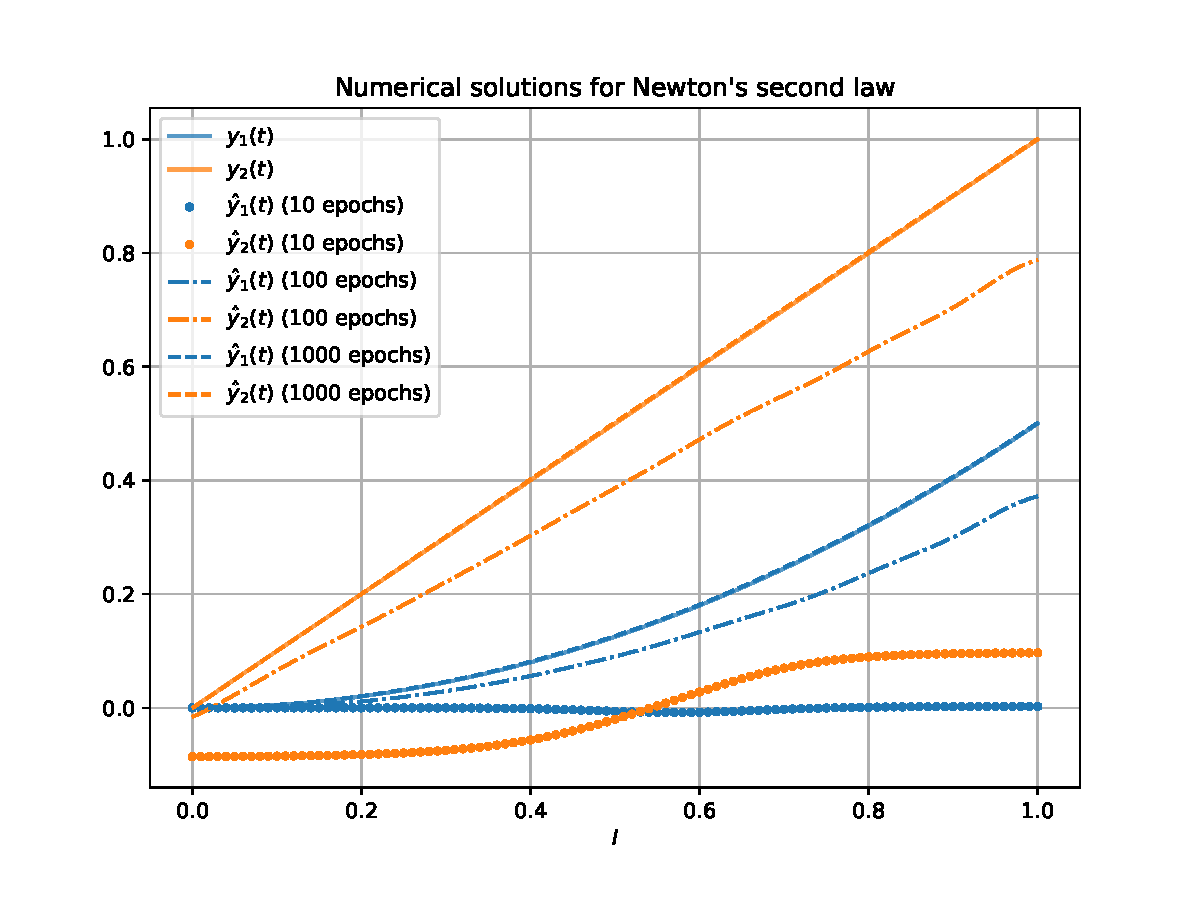
\includegraphics[width=0.8\textwidth]{images/pinn_newton.pdf}
    \caption[Performance of a \gls{PINN} in comparison to \gls{RK4} in solving an \gls{IVP} of Newton's second law]{Performance of a \gls{PINN} in comparison to \gls{RK4} in solving an \gls{IVP} of Newton's second law for $I=\left[ 0,1 \right] $. In the graphic, $y_1$ and $y_2$ are the results of the numerical solver, while $\hat{y}_1$ and $\hat{y}_2$ are the results of the \gls{PINN} trained after different numbers of epochs. \gls{PINN} results for 1000 epochs overlap \gls{RK4} results.}
    \label{fig:images-pinn_newton-pdf}
\end{figure}

